\section{Deep Reinforcement Learning}
\subsection{Fundamentals of Reinforcement Learning}
\begin{itemize}
	\begin{figure}[ht!]
		\centering
		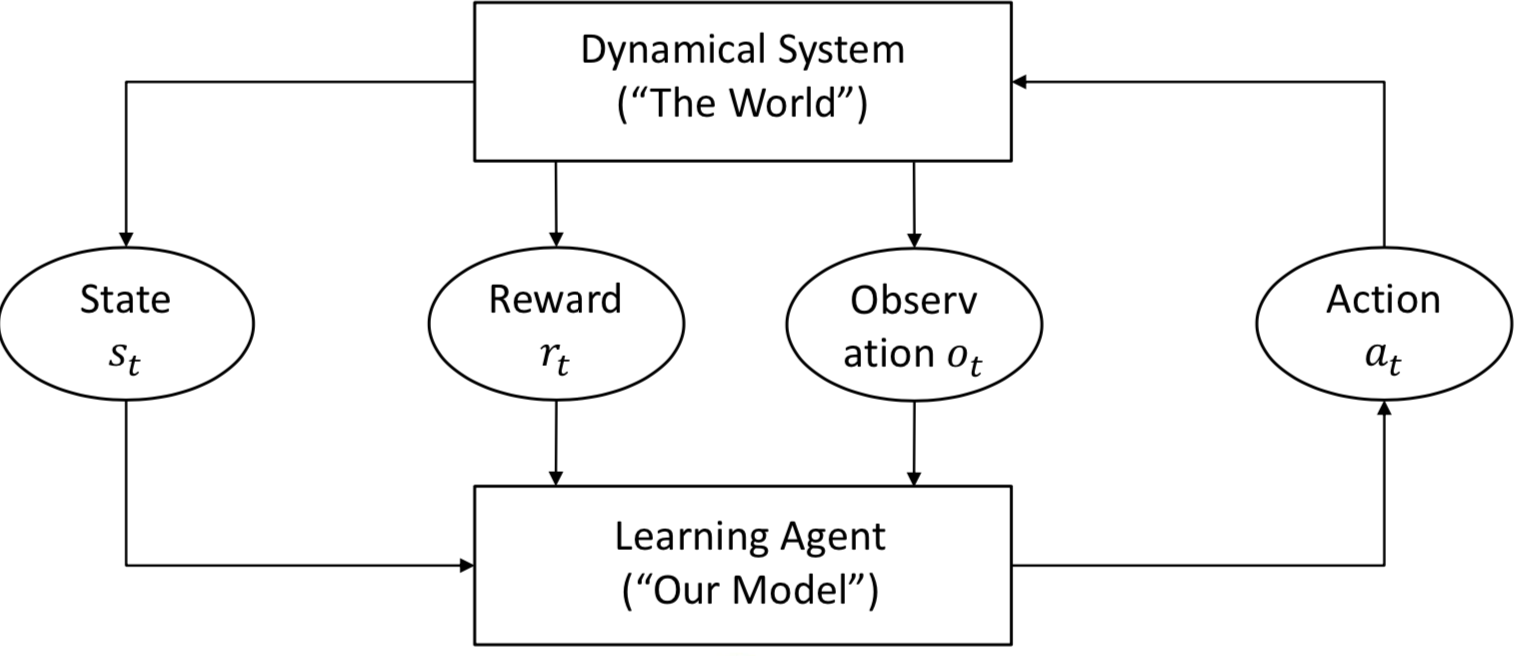
\includegraphics[width=0.4\textwidth]{figures/RL_basic_concept.png}
		\caption{Interaction model between environment and agent}
	\end{figure}
	\item The \textbf{state} $s_t$ is the summary of all experience so far: $s_t = f(o_1, r_1, a_1, o_2, r_2, a_2, ..., o_t, r_t)$ ($o_i$ observable part of environment at time step $i$). If we have a fully observable environment, then $s_t = f(o_t)$.
	\item The \textbf{policy} of an agent determines its actions: $\pi\left(a_t|s_t\right)$. Can be deterministic or stochastic
	\item The \textbf{value function} is the expected total reward under policy $\pi$: $$q^{\pi}(s_t, a_t) = \mathbb{E}_{\pi}\left[r_{t+1}+\gamma r_{t+2} + \gamma^2 r_{t+3} + ... | s_t, a_t\right]$$
	$\gamma$ as discount factor as we are most certain about close rewards and sometimes are more interested in immediate rewards
	\item \textbf{Bellman equation} for value function:
	$$q^{\pi}(s_t, a_t) = \mathbb{E}_{s', a'}\left[r + \gamma q^{\pi}\left(s', a'\right) | s_t, a_t\right] = \sum_{s'} p(s'|s_t,a_t)\cdot \left[r(s', a_t, s_t) + \gamma \sum_{a'} \pi(a'|s') \cdot q^{\pi}\left(s', a'\right) \right]$$
	\item The optimal value function is therefore $q^{*}(s_t,a_t) = \max_{\pi} q^{\pi}(s_t,a_t) = r_{t+1} + \gamma \max_{a_{t+1}}$
	\item The \textbf{environment} can be modeled by the agent (learned from experience), and used for planning and look ahead. This can be for example a simulator
\end{itemize}
\subsection{Deep RL approaches}
\subsubsection{Value-based approaches}
\begin{itemize}
	\item Try to learn value function $q^*$ to get the optimal policy $\pi^*$
	\item The input to such models is usually the state, which should be as raw as possible (e.g. image frames). We can either add the action to the input and let the network predict its Q-value, or predict Q-values for all possible actions (second is faster and simpler)
	\begin{figure}[ht!]
		\centering
		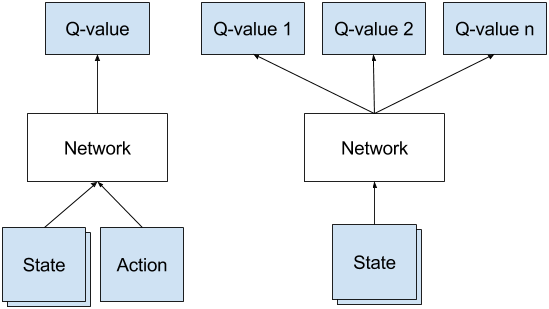
\includegraphics[width=0.4\textwidth]{figures/RL_deep_QLearning.png}
		\caption{Modeling of Q-value predictions}
	\end{figure}
	\item Optimization by SARSA-like loss:
	$$\mathcal{L} = \mathbb{E}\left[\left(r + \gamma \max_{a_{t+1}} q(s_{t+1}, a_{t+1}, \theta) -q(s_{t}, a_{t}, \theta) \right)^2\right]$$
	\item For the gradients, we assume that the bootstrapped max value is fixed:
	$$\pd{\mathcal{L}}{\theta} = \mathbb{E}\left[-2\cdot \left(r + \gamma \max_{a_{t+1}} q(s_{t+1}, a_{t+1}, \theta) -q(s_{t}, a_{t}, \theta) \right) \cdot \pd{q(s_{t}, a_{t}, \theta)}{\theta}\right]$$
	\item Optimize with SGD by sampling one action and state, calculate q-values for all possible future actions, and use the maximum as bootstrap goal
\end{itemize}
\subsubsection{Stability problems}
\begin{itemize}
	\item As we bootstrap, the target is always changing $\Rightarrow$ policy changes fast, can lead to oscillations
	\item The sequential data breaks the iid assumption on which SGD relies
	\item The scale of Q-values is not easy to control, and is very task dependent $\Rightarrow$ gradients are unstable and can be either too large or too small
	\item \textbf{Improving stability}
	\begin{itemize}
		\item \textit{Experience replay}: store memories of $\langle s, a, r, s'\rangle$ (with e.g. a $\epsilon$-greedy policy) in a dataset, and sample batches from there to train on. Breaks temporal dependency and helps SGD by i.i.d.
		\item \textit{Freezing target}: instead of having a moving target, we freeze the $Q$ network every $K$ iterations, and use that to generate our targets (Q-targets come now from a bit older network parameter setting, but is steady over $K$ iterations). Avoids oscillations
		\item \textit{Clipping rewards}: Normalize or clip rewards to be in range $[-1,+1]$ or any other stable range. Prevents unknown scales of $Q$
		\item \textit{Skipping frames}: a light version of experience replay is skipping $N$ frames between two data points to avoid too strong temporal dependency (two consecutive frames are very similar)
		\item \textit{Exploration vs Exploitation}: use a $\epsilon$-greedy policy with annealing temperature. In the beginning, we will focus on exploration while slowly converging to exploitation
	\end{itemize}
\end{itemize}
\subsubsection{Policy-based approaches}
\begin{itemize}
	\item Try to learn the optimal policy $\pi^*$ directly from experience (parameterized policy $\pi_w(a_t|s_t)$)
	\item Avoids learning the $q$ values which are hard for continuous action spaces, and tend to oscillate because of bootstrapping
	\item Training steps
	\begin{enumerate}
		\item Determine Q-value for current policy by running a simulation:\\ $q^{\pi_w}(s_t, a_t) = \mathbb{E}\left[r_t + \gamma r_{t+1} + \gamma^2 r_{t+2} + ... | \pi_{w}\right]$
		\item Maximize q-values as loss function. 
		\begin{enumerate}
			\item If policy is deterministic:
			$$\pd{\mathcal{L}}{w} = \mathbb{E}\left[\chain{q^{\pi}(s,a)}{a}{w}\right]$$
			\item If policy is stochastic:
			$$\pd{\mathcal{L}}{w} = \mathbb{E}\left[\pd{\log \pi^{w}(a|s)}{w} q^{\pi}(s,a)\right]$$
		\end{enumerate}
	\end{enumerate}
	\item Asynchronous Advantage Actor-Critic
	\begin{itemize}
		\item Learn both policy and value function
		\item Multiple agents that simultaneously interact with (copy of) environment and learn
		\item \textit{Advantage estimates}: Use the learned value function to compare to your actually gained $q$ value. Loss is therefore higher if unexpected things happen $\Rightarrow$ exploration
	\end{itemize}
	\begin{figure}[ht!]
		\centering
		\begin{subfigure}{0.45\textwidth}
			\centering
			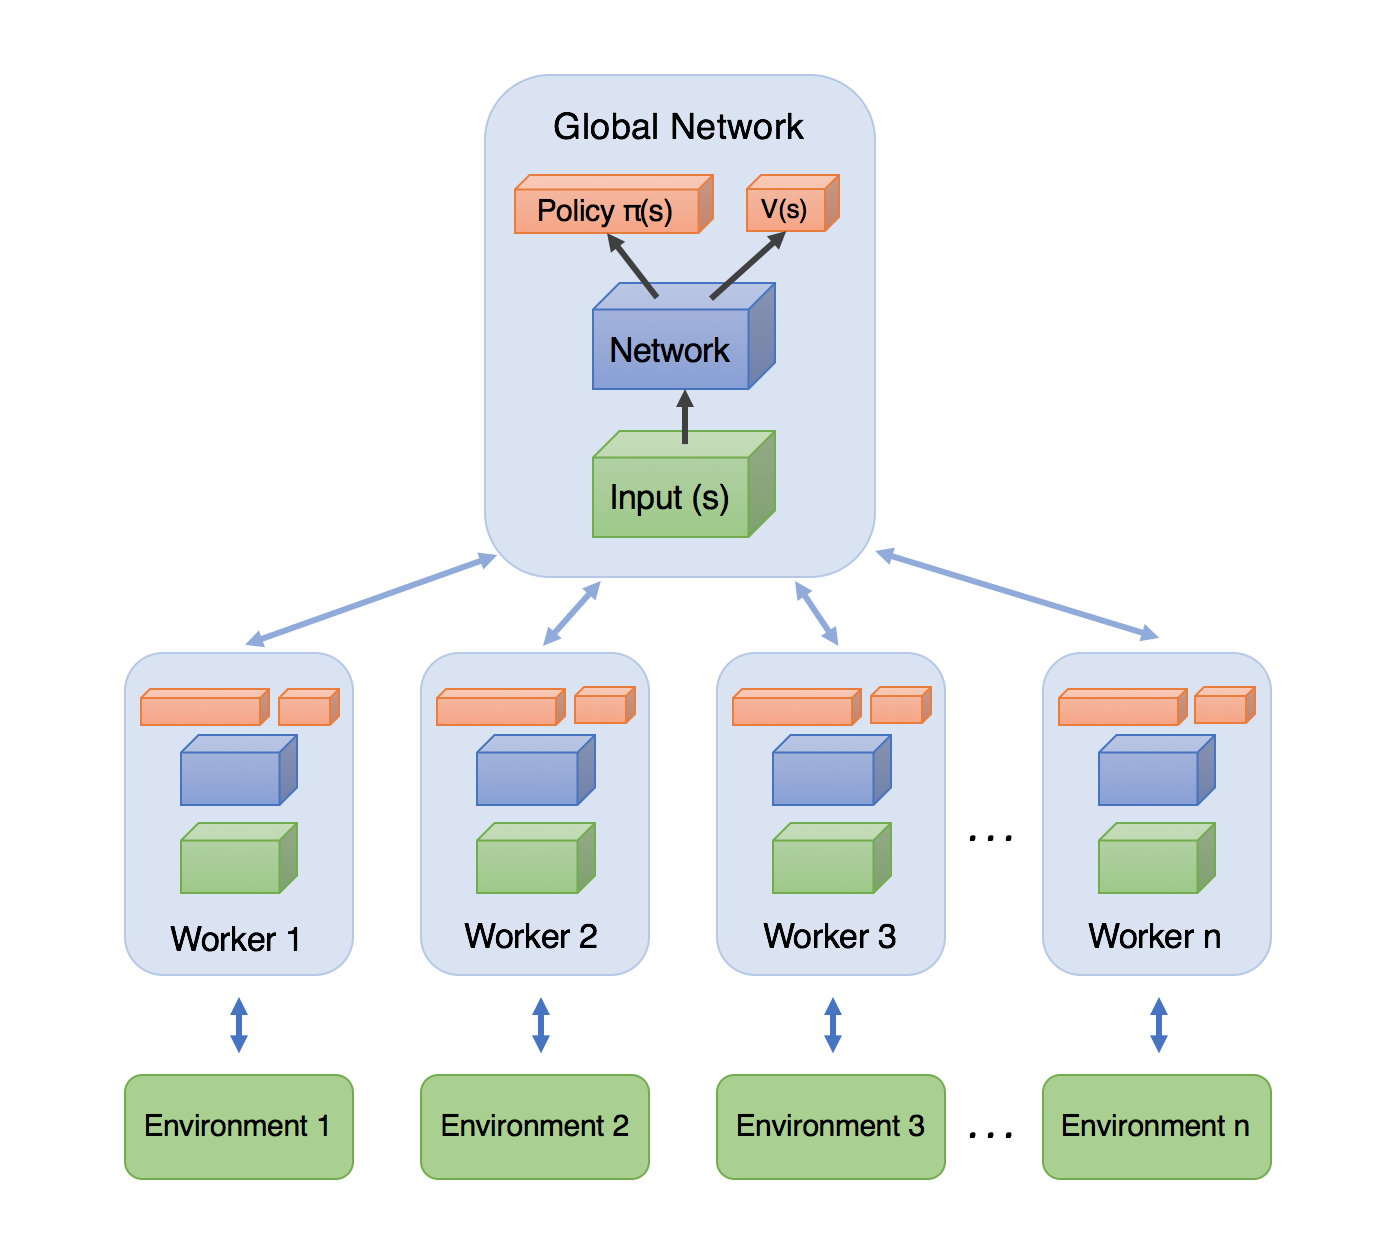
\includegraphics[width=0.8\textwidth]{figures/RL_A3C_multiple_workers.png}
		\end{subfigure}
		\begin{subfigure}{0.45\textwidth}
			\centering
			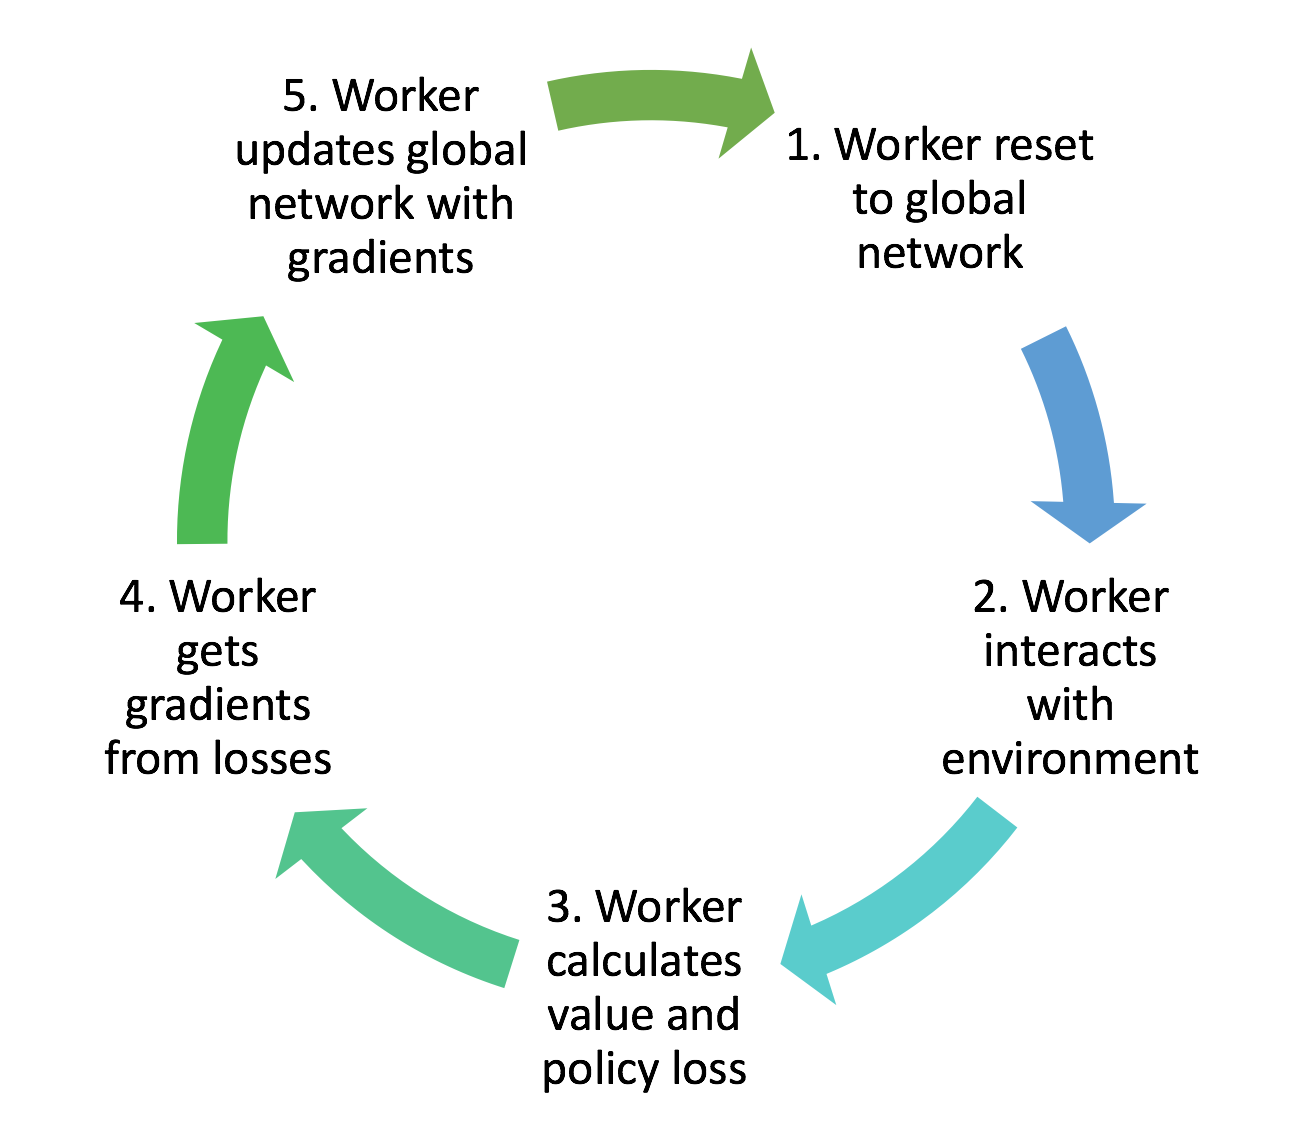
\includegraphics[width=0.8\textwidth]{figures/RL_A3C_cycle.png}
		\end{subfigure}
		\caption{Schematic overview of A3C}
		\label{fig:RL_A3C}
	\end{figure}
\end{itemize}
\subsubsection{Model-based approaches}
\begin{itemize}
	\item Try to model the environment to be aware of rules etc. 
	\item Example: AlphaGo relies on Tree-Search guided by CNNs. We use two policy networks to play against each other, and one value network that predicts the value function of a state
\end{itemize}